% !TEX root = ../../prj4projektdokumentation.tex

\subsection{Analog til digital konvertering}

Måleenheden omsætter to analoge spændingssignaler til digitale værdier for strøm og spænding. Denne konvertering foretages af en Delta Sigma Analog to Digital Converter (ADC) i PSOCen, se datablad for ADC i bilag A1.  ADC er en komponent i PSOC, som med en read-funktion kan returnere en 16-bit værdi af det analoge signal på indgangen. 

På Figur \ref{fig:MEADC} ses blokkaldet i PSOC creator 4.0. Blokken er sat op med følgende parametre:
\begin{align}
Resolution = 16bit
\end{align}
\begin{align}
f_{sample} = 41666 Hz
\end{align}

\begin{figure}[htbp] % (alternativt [H])
	\centering
	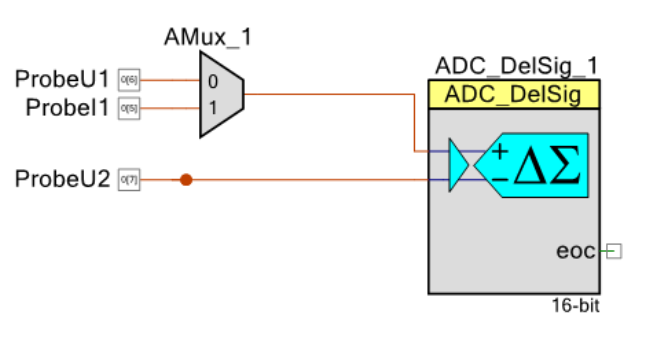
\includegraphics[width=0.6\textwidth]{Figure/MEADC}
	\caption{ADC blok fra PSOC creator 4.0}
	\label{fig:MEADC}
\end{figure}

Som det fremgår af Figur \ref{fig:MEADC} er der anvendt 2 multiplexere, til at skifte mellem hvilke signaler der skal samples. Dette skyldes at der kun er én ADC i PSOCen. Samplingen af signalet styres i C-koden, hvor der anvendes to af ADC-blokkens API funktioner. 
\\

\textbf{GetResult16() }starter en ADC konvertering, venter på at denne er færdig, stopper konverteringen og returnerer en 16bit signed integer værdi af resultatet. 
\\

\textbf{CountsTo\_mVolt()} konverterer resultatet af GetResult16() til en værdi i millivolt. 
\\

Koden til sampling af signalerne er vist grafisk i et flowchart på Figur \ref{fig:MEsample}. Samplingen kører i en for-løkke, hvor der skiftevis tages et sample af spændingen og strømmen. Efter hvert andet sample, indføres der et delay, således at sampletiden passer med én periode af et 50Hz sinussignal. Antallet af samples er 64 pr. signal, altså 128 i alt. De samplede værdier gemmes i to arrays, som bruges i de efterfølgende beregninger. 


\begin{figure}[htbp] % (alternativt [H])
	\centering
	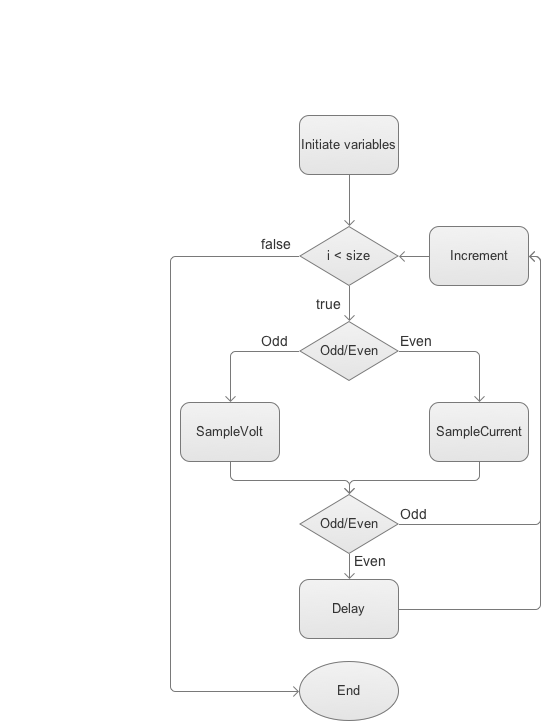
\includegraphics[width=0.6\textwidth]{Figure/MEsample}
	\caption{Flowchart for sample funktionen i PSOC}
	\label{fig:MEsample}
\end{figure}

\subsubsection{Realisering af samplefrekvens}

Det indførte delay i for-løkken skal sikre at sampletiden svarer præcist til én periode af et 50Hz sinussignal.
\begin{align}
T_{sample} = \frac{1}{50Hz} = \SI{20}{\milli\second}
\end{align}

Det betyder at tiden mellem hvert sample skal være
\begin{align}
t = \frac{T_{sample}}{128} = \SI{156,25} {\micro\second}
\end{align}

Den reelle tid der er mellem samples afhænger af hvor lang tid det tager at eksekvere koden på PSOC. Denne tid er fundet ved at toggle et testben på PSOC, før og efter samplingen, og anvende Analog Discoverys Logic Analyser til at måle tiden. Tiden det tager at tage et sample fra hvert signal er aflæst til: $t_{reel} = \SI{131,81}{\micro\second}$.  Herefter kan størrelsen på delayet udregnes.
\begin{align}
resttid = T - (t_{reel}*64) = \SI{11,564}{\milli\second}
\end{align}
\begin{align}
delay = \frac{resttid}{64} = \SI{180,69} {\micro\second}
\label{eq:MEdelay}
\end{align}

Dette delay indsættes i koden og Logic Analyser bruges til at finde den reelle sampletid, som findes til $T_{sampleReel} = \SI{29,131}{\milli\second}$, se Figur \ref{fig:MEsampleTest1}.

\begin{figure}[htbp] % (alternativt [H])
	\centering
	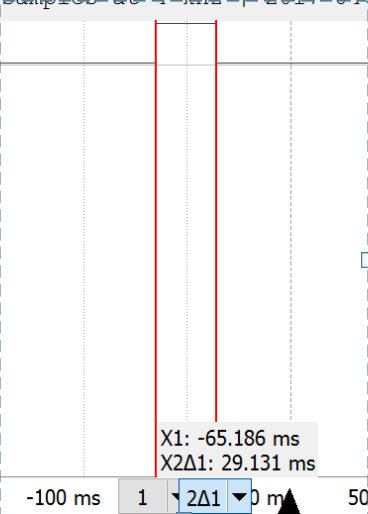
\includegraphics[width=0.3\textwidth]{Figure/MEtestSample1}
	\caption{Reel sampletid med beregnet delay, fundet med Logic Analyser}
	\label{fig:MEsampleTest1}
\end{figure}

Det viser sig at delayet er blevet for stort. Derfor laves endnu en beregning, hvor denne fejl fratrækkes delayet fra (\ref{eq:MEdelay}).
\begin{align}
delay_2 = delay - \frac{\SI{29.131}{\milli\second}-\SI{20}{\milli\second}}{64} = \SI{38,018} {\micro\second}
\end{align}

Ved at indsætte dette delay, kommer sampletiden meget tæt på de $\SI{20}{\milli\second}$, og med småjusteringer af delayet, findes den rigtige værdi til $\SI{40}{\micro\second}$, se Figur \ref{fig:MEsampleTest2}, hvor sampletiden er aflæst til $\SI{20,057}{\milli\second}$.

\begin{figure}[H] % (alternativt [H])
	\centering
	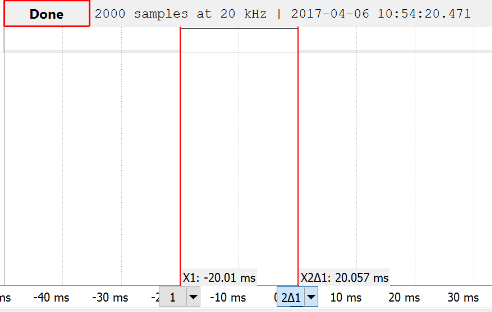
\includegraphics[width=0.6\textwidth]{Figure/MEtestSample2}
	\caption{Reel sampletid med endeligt delay, fundet med Logic Analyser}
	\label{fig:MEsampleTest2}
\end{figure}


